\documentclass[a4paper]{article}
\usepackage[width=15cm,height=25.7cm]{geometry}
\usepackage{xspace}
\usepackage{color}
\usepackage[leqno]{amsmath}
\usepackage{amssymb}
\usepackage{array}
\usepackage{tabularx}
\usepackage{booktabs}
\usepackage{url}
\usepackage{hyperref}
\usepackage{breakurl}
\usepackage{graphicx}
\usepackage{subfigure}
\usepackage[draft]{fixme}
\def\url@leostyle{%
  \@ifundefined{selectfont}{\def\UrlFont{\small\sf}}{\def\UrlFont{\small\sf}}}
\makeatother
\urlstyle{leo}
\usepackage[normalem]{ulem}
\usepackage{xspace}
%same notation policy for each instance of figure, thm, etc
\newcommand{\myfig}{Fig.~}
\newcommand{\mytab}{Tab.~}
\newcommand{\mysec}{Sec.~}
\newcommand{\mychap}{Chap.~}
\newcommand{\myapp}{App.~}
\newcommand{\etal}{et~al.\xspace}
\newcommand{\wrt}{w.r.t.\xspace}
\newcommand{\eg}{e.g.\xspace}
\newcommand{\ie}{i.e.\xspace}
\newcommand{\etc}{etc.\xspace}
\newcommand{\cf}{see\xspace}

%les maths comme au lycee
\let\eset\emptyset
\newcommand{\rplus}[1]{\mathop{{#1}^{+}}}
\newcommand{\rstar}[1]{\mathop{{#1}^{*}}}
\newcommand{\transc}[1]{\mathop{{#1}^{+}}}
\newcommand{\maybe}[1]{\mathop{{#1}^{?}}}

%def
  \newcommand{\dfnshort}[2]{{#1}\triangleq{#2}}
  \newcommand{\dfn}[2]{{#1}~\triangleq~{#2}}

%sets
\newcommand{\setcal}[1]{\mathcal{#1} }
\newcommand{\setbf}[1]{\mathbb{#1} }
\newcommand{\setfrak}[1]{\mathfrak{#1} }


  %writes, reads, barriers
  \let\setset\setbf
  \newcommand{\evts}{\setset{E}}

  \newcommand{\lwf}{\textsf{fence}}
  \newcommand{\mfence}{\ensuremath{\mathsf{mfence}}}
  \newcommand{\lwfence}{\ensuremath{\mathsf{fence}}}
  \newcommand{\ff}{\textsf{fence.sc}}
  \newcommand{\ffence}{\ensuremath{\mathsf{f{\kern-0.1em}fence}}}
  \newcommand{\fences}{\ensuremath{\mathsf{fence}}}
  \newcommand{\relw}{\ensuremath{\mathsf{rel}}}
  \newcommand{\acqr}{\ensuremath{\mathsf{acq}}}
  \newcommand{\cumul}{\ensuremath{\mathsf{cumul}}}
  \newcommand{\Acumul}{\ensuremath{\mathsf{A{\kern-0.3em}-{\kern-0.3em}cumul}}}

  %procs
  \newcommand{\pr}{\operatorname{proc}}

  %locs
  \newcommand{\lo}{\ell}
  \newcommand{\loc}{\operatorname{addr}}

  %vals 
  \newcommand{\val}{\operatorname{val}}

%relations
\newcommand{\stacklabel}[1]
%{\stackrel{\smash{\scriptscriptstyle\#1}}}
{\stackrel{\smash{\scriptstyle\textnormal{#1}}}}
  %any
  \newcommand{\rln}[1]{\ensuremath{\xrightarrow{#1}}}

  %po
  \newcommand{\iico}{\ensuremath{\mathsf{ii}}}
  \newcommand{\ctrlcfence}{\ensuremath{\mathsf{ctrlcfence}}}
  \newcommand{\ctrl}{\ensuremath{\mathsf{ctrl}}}
  \newcommand{\data}{\ensuremath{\mathsf{data}}}
  \newcommand{\addr}{\ensuremath{\mathsf{addr}}}
  \newcommand{\ddreg}{\ensuremath{\mathsf{dd}}}
  \newcommand{\rfreg}{{\mathsf{rfreg}}}
  \newcommand{\isb}{\ensuremath{\mathsf{isb}}}
  \newcommand{\isync}{\ensuremath{\mathsf{isync}}}
  \newcommand{\po}{\ensuremath{\mathsf{po}}}
  \newcommand{\ppo}{\ensuremath{\mathsf{ppo}}}
  %rf
  \newcommand{\rf}{\ensuremath{\mathsf{rf}}}
  %rfe
  \newcommand{\rfe}{\ensuremath{\mathsf{rfe}}}
  %rfi
  \newcommand{\rfi}{\ensuremath{\mathsf{rfi}}}
  %co
  \newcommand{\co}{\ensuremath{\mathsf{co}}}
  \newcommand{\coi}{\ensuremath{\mathsf{coi}}}
  \newcommand{\ews}{\ensuremath{\mathsf{coe}}}
  %fr
  \newcommand{\fr}{\ensuremath{\mathsf{fr}}}
  \newcommand{\ifr}{\ensuremath{\mathsf{fri}}}
  \newcommand{\efr}{\ensuremath{\mathsf{fre}}}
  %hb
  \newcommand{\com}{\ensuremath{\mathsf{com}}}
  \newcommand{\cause}{\ensuremath{\mathsf{cause}}}
  \newcommand{\hb}{\ensuremath{\mathsf{hb}}}
\newcommand{\propbase}{\operatorname{\ensuremath{\mathsf{prop{\kern-0.00em}-{\kern-0.1em}base}}}}
\newcommand{\prop}{\operatorname{\ensuremath{\mathsf{prop}}}}
  %poloc
  \newcommand{\polocllh}{\operatorname{\ensuremath{\mathsf{po{\kern-0.00em}-{\kern-0.1em}loc{\kern-0.00em}-{\kern-0.05em}llh}}}}
  \newcommand{\poloc}{\operatorname{\ensuremath{\mathsf{po{\kern-0.00em}-{\kern-0.05em}loc}}}}
  %criteria
  \newcommand{\acyclic}{\operatorname{acyclic}}
  \newcommand{\reflexive}{\operatorname{reflexive}}
  \newcommand{\irrefl}{\operatorname{irreflexive}}
  %po restricted to some events
  \newcommand{\WW}{\operatorname{\ensuremath{\mathsf{{WW}}}}}
  \newcommand{\RM}{\operatorname{\ensuremath{\mathsf{RM}}}}
  \newcommand{\RW}{\operatorname{\ensuremath{\mathsf{RW}}}}
  \newcommand{\RR}{\operatorname{\ensuremath{\mathsf{RR}}}}
  \newcommand{\RB}{\operatorname{\ensuremath{\mathsf{RB}}}}
  \newcommand{\MW}{\operatorname{MW}}
  \newcommand{\WM}{\operatorname{WM}}
  \newcommand{\WR}{\operatorname{\ensuremath{\mathsf{WR}}}}

\newcommand{\wide}{wide}
\newcommand{\wider}{wider}
\newcommand{\widest}{widest}
\newcommand{\narrow}{narrow}
\renewcommand{\narrower}{narrower}
\newcommand{\narrowest}{narrowest}
\newcommand{\narrowerop}{\operatorname{narrower}}

%%%Litmus
%%basic format
\let\prog\textsf
\let\as\texttt
\let\ltest\textbf

%% Conventional processor
\newcommand{\proc}[1]{\ensuremath{P_{#1}}}
%% Format graphs in columns
\makeatletter
\@ifundefined{useepstrue}{\newif\ifuseeps\useepsfalse}{}
\makeatother
\newlength{\fmtlength}
\ifuseeps
\newcommand{\fmtgraphcol}[3]
{\setlength{\fmtlength}{\linewidth}%
\addtolength{\fmtlength}{-#2}%
\framebox{\resizebox{\fmtlength}{#3}{\includegraphics{#1.eps}}}}
\else
\newcommand{\fmtgraphcol}[3]
{\setlength{\fmtlength}{\linewidth}%
\addtolength{\fmtlength}{-#2}%
\framebox{\resizebox{\fmtlength}{#3}{\input{#1.pstex_t}}}}
\fi
%%Format graph explicit width
\ifuseeps
\newcommand{\fmtgraph}[3]
{\resizebox{#2}{#3}{\includegraphics{#1.eps}}}
\newcommand{\tfmtgraph}[1]{\framebox{\includegraphics{#1.eps}}}
\else
\newcommand{\fmtgraph}[3]
{\resizebox{#2}{#3}{\input{#1.pstex_t}}}
\newcommand{\tfmtgraph}[1]{\framebox{\input{#1.pstex_t}}}
\fi
%%%%Test for figures as in the tutorial
% fix up fig2dev fonts to make actions in \sf
\iftrue
\makeatletter
% for the fig2dev version on P laptop
\gdef\SetFigFontNFSS#1#2#3#4#5{%
  \reset@font\fontsize{#1}{#2pt}%
%  \fontfamily{#3}\fontseries{#4}\fontshape{#5}%
  \fontfamily{\sfdefault}\fontseries{#4}\fontshape{#5}%
  \selectfont}%
% for the fig2dev version on P desktop
\gdef\SetFigFont#1#2#3#4#5{%
  \reset@font\fontsize{#1}{#2pt}%
%  \fontfamily{#3}\fontseries{#4}\fontshape{#5}%
  \fontfamily{\sfdefault}\fontseries{#4}\fontshape{#5}%
  \selectfont}
\makeatother
\newcommand{\asm}[1]{\texttt{#1}}
\newcommand{\myth}[1]{\ensuremath{\mathsf{T}_#1}}
\newcommand{\mylegend}[2]{#1}
\ifbw\newcommand{\bw}{-bw}\else\newcommand{\bw}{}\fi
\ifuseeps
\newcommand{\locfmt}[1]{\includegraphics{#1.eps}}
\newcommand{\newfmt}[1]{\includegraphics{img/#1.eps}}
\newcommand{\insfmt}[1]{\scalebox{0.28}{\includegraphics{ins/#1.eps}}}
\else
\newcommand{\locfmt}[1]{\input{#1.pstex_t}}
\newcommand{\newfmt}[1]{\input{img/#1\bw.pstex_t}}
\newcommand{\insfmt}[1]{\scalebox{0.28}{\input{ins/#1\bw.pstex_t}}}
\fi
\fi

\newcommand{\NEW}[1]{\textcolor{blue}{#1}}

\newcolumntype{Y}{@{}r@{\,}X}
%%Decorate instruction with a label
\newcommand{\instab}[2]{\ \(#2\)  & \as{#1}}
%%Pseudo-code load & store
\newcommand{\pset}[2]{\(\as{#1} \leftarrow \as{#2}\)}
\newcommand{\pstore}[2]{\pset{#2}{#1}}
\newcommand{\pload}[2]{\pset{#1}{#2}}
%%trick to add vertical space somewhere
\newcommand{\haut}{\rule{0ex}{2ex}}
\newcommand{\bas}{\rule[-1ex]{0.5ex}{0ex}}



\title{A note on the Linux model}
\date{}
\author{Jade Alglave}
\begin{document}
\maketitle

Our Linux model is phrased in terms of \emph{events} (e.g. reads and writes),
and relations over these events (e.g. program order, read-from \dots).

\section{Events}

Events can be \emph{accesses} (e.g. reads and writes), or \emph{fences} (e.g.
{\tt wmb, rmb} \dots).

\subsection{Accesses}

\begin{verbatim}
enum Accesses = 'once ||
                'release || 'acquire ||
                'assign || 'deref || 'lderef 
events R[{'once,'acquire,'deref,'lderef}]
events W[{'once,'release,'assign}]
\end{verbatim}

Our accesses can be reads or writes, bearing \emph{annotations}. A read can
bear:
\begin{itemize}
\item {\tt 'once}, corresponding to {\tt READ\_ONCE};
\item {\tt 'acquire}, making it a read acquire;
\item {\tt 'deref}, corresponding to {\tt rcu\_dereference};
\item {\tt 'lderef}, corresponding to {\tt lockless\_dereference}.
\end{itemize}

A write can bear:
\begin{itemize}
\item {\tt 'once}, corresponding to {\tt WRITE\_ONCE};
\item {\tt 'release}, making it a write release;
\item {\tt 'assign}, corresponding to {\tt rcu\_assign\_pointer}.
\end{itemize}

\subsection{Fences}

\subsubsection{Annotations on fence events}

\begin{verbatim}
enum Barriers = 'wmb || 'rmb || 'mb
                || 'rb_dep
                || 'lock || 'unlock 
                || 'sync 
events F[Barriers]
\end{verbatim}

Fences can bear:
\begin{itemize}
\item {\tt 'wmb}, i.e. be a write memory barrier;
\item {\tt 'rmb}, i.e. be a read memory barrier;
\item {\tt 'mb}, i.e. be a full memory barrier;
\item {\tt 'rb\_dep}, corresponding to {\tt smp\_read\_barrier\_depends};
\item {\tt 'lock}, corresponding to {\tt rcu\_read\_lock};
\item {\tt 'unlock}, corresponding to {\tt rcu\_read\_unlock};
\item {\tt 'sync}, corresponding to {\tt synchronize\_rcu}.
\end{itemize}

\subsubsection{Relations induced by fences}

For each user-defined annotation {\tt 't}, \prog{herd} defines a set {\tt T} of
all events bearing this annotation. Thus {\tt Rmb} is the set of all events
bearing the annotation {\tt 'rmb}. Using these sets, we can define the ordering
relations induced by a given fence for example. 

To do so, we rely on the {\tt fencerel} function from the standard library of
\prog{herd}. The function {\tt fencerel} takes as argument a set {\tt S}, and
gathers all pairs of events in program order that have an element of {\tt S} in
between them in {\tt po}:
\begin{verbatim}
let fencerel(S) = (po & (_ * S)) ;  po
\end{verbatim}

So now we can define the relations {\tt rmb, wmb, mb} and {\tt sync}, eponymous
of the fence events' annotations:
\begin{verbatim}
let rmb = fencerel(F & Rmb) & (R*R)
let wmb = fencerel(F & Wmb) & (W*W)
let mb = fencerel(F & Mb)
let sync = fencerel(F & Sync)
\end{verbatim}

As one can see, {\tt rmb} is the relation between two read events (observe the
intersection {\tt \&} with the read-read pairs {\tt R*R}) in program order
separated by a fence event (i.e. from the predefined set {\tt F}) bearing the
annotation {\tt 'rmb}. Similarly, {\tt wmb} is the relation between two write
events in program order separated by a fence event bearing the annotation {\tt
'wmb}. The relations {\tt mb} and {\tt sync} are between events in program
order separated by a fence event bearing the annotation {\tt 'mb} and {\tt
'sync} respectively. 

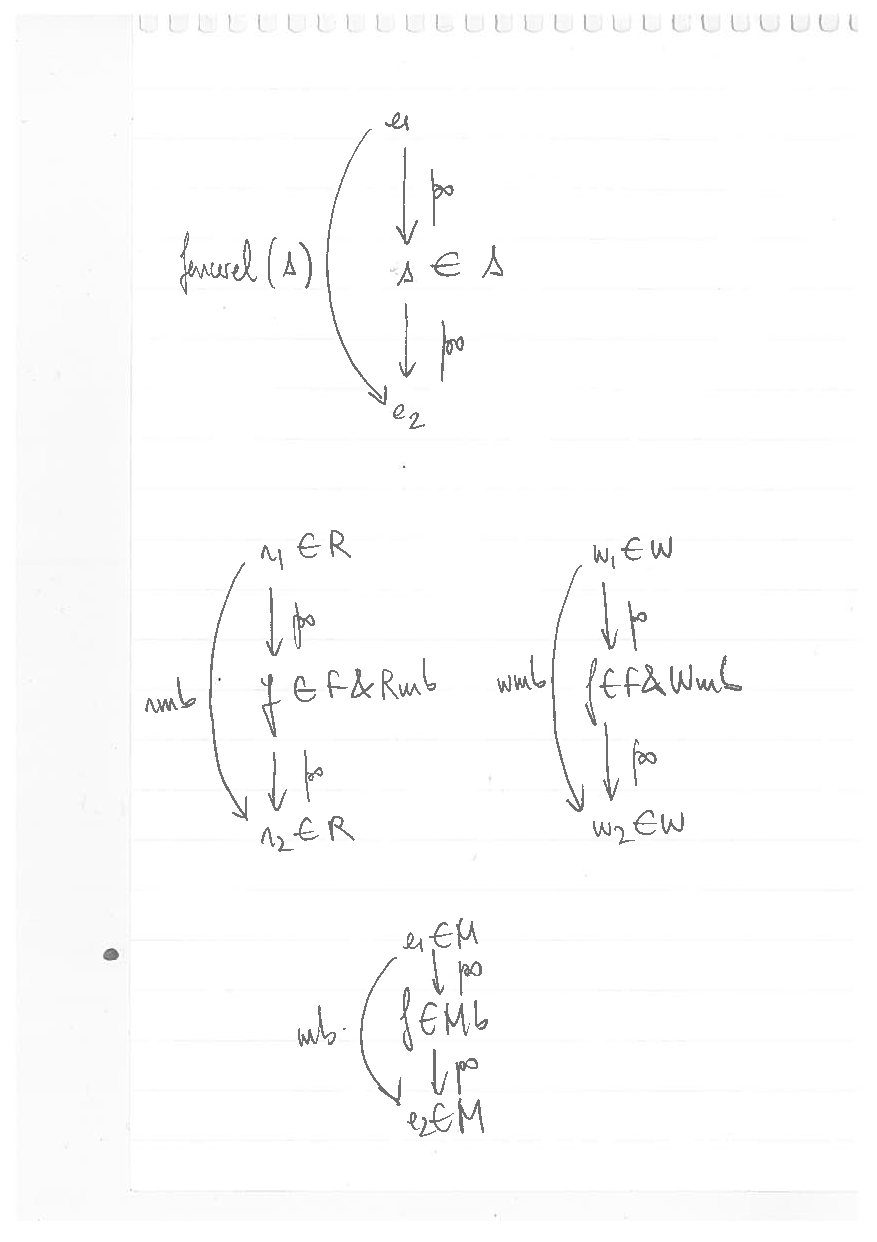
\includegraphics[width=11cm]{fencerel}

\pagebreak
Finally, the relation {\tt fences} is made of the union of
all these relations:
\begin{verbatim}
let fences = rmb | wmb | mb | sync
\end{verbatim}

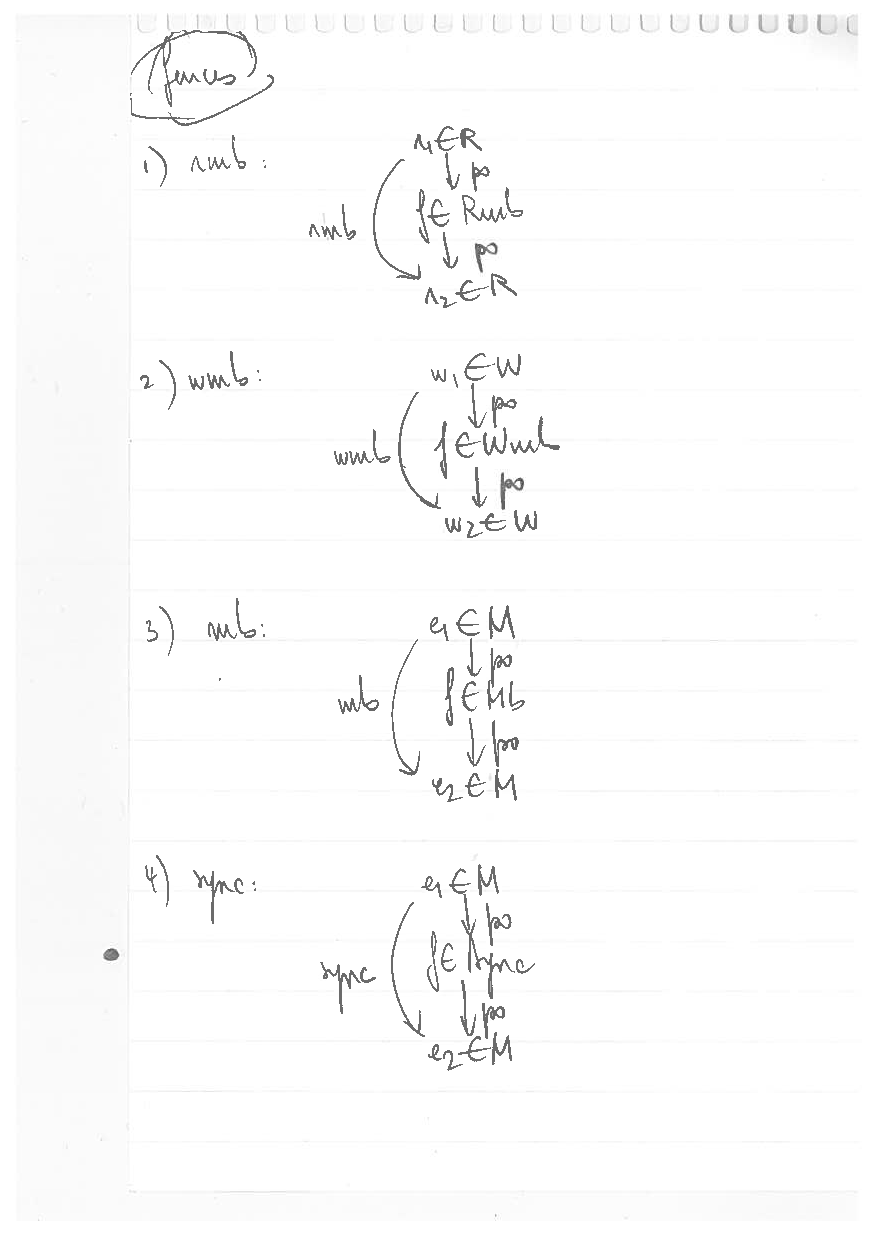
\includegraphics[width=11cm]{fences}

\pagebreak

\subsubsection{Relations induced by special accesses}

For each user-defined annotation {\tt 't}, \prog{herd} defines a set {\tt T} of
all events bearing this annotation. Thus {\tt Assign} is the set of all events
bearing the annotation {\tt 'assign}. Using these sets, we can define the
ordering relations induced by special accesses for example. 

The following relations restrict the set of pairs in program order to one
extremity being special, e.g. {\tt acq-po} requires that the left extremity
bears the annotation {\tt 'acquire} (i.e. is a read acquire), and {\tt
po-assign} requires that the right extremity bears the annotation {\tt 'assign}
(i.e. is an {\tt rcu\_assign\_pointer}):
\begin{verbatim}
let acq-po = po & (Acquire * M)
let po-rel = po & (M * Release)

let deref-po = po & (Deref * M)
let lderef-po = po & (Lderef * M)
let po-assign = po & (M * Assign)

let lock-po = po & (Lock * M)
let po-unlock = po & (M * Unlock)
\end{verbatim}

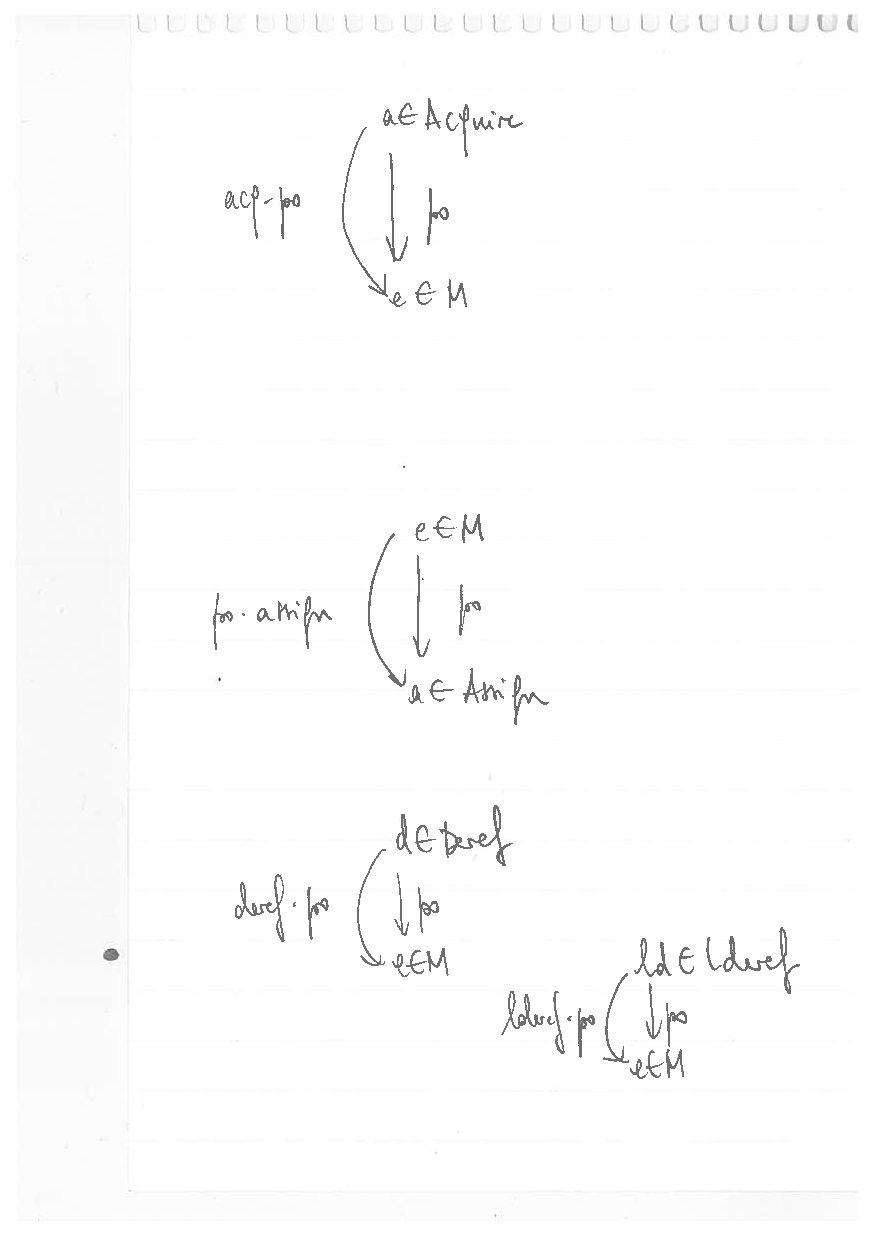
\includegraphics[width=12cm]{acq-po}

\section{Relations and axioms}

\subsection{Communications and SC per location}

\begin{verbatim}
let po-loc = po & loc
let com = rf | co | fr
\end{verbatim}

In {\tt po-loc} we gather the \emph{program order} {\tt po} restricted to
accesses of the same memory location or variable: the relation {\tt loc}
gathers all pairs of accesses to the same location, so that the intersection
{\tt \&} of {\tt po} and {\tt loc} creates the set of pairs of accesses in
program order and relative to the same location. In {\tt com} we gather the
\emph{communication} relations, i.e. read-from {\tt rf}, coherence {\tt co} and
from-read {\tt fr}.

The procedure {\tt sc-per-location} ensures that these two relations are in
accord:
\begin{verbatim}
procedure sc-per-location() =
  let order = po-loc | com
  acyclic order
end
\end{verbatim}

This procedure creates a relation {\tt order} made of the union of {\tt po-loc}
and {\tt com}, and requires its acyclicity, effectively making it an order.

\subsection{Stitches}

Our Linux model is made of two kinds of \emph{stitches} (i.e. combinations of
relations): non-transitive and transitive ones. We'll use our stitches in
various ways to build the two main relations of our model, namely the
happens-before relation {\tt hb}, and the propagation order {\tt prop}. 

\subsubsection{Local and non-transitive stitches\label{sec:local}}

The first kind of stitch is \emph{non-transitive}. It is made of
\emph{dependencies}, in combination with certain special accesses and fences,
and one optional step of read-from.

More precisely we define the relation {\tt deps} as the union of \emph{address}
{\tt addr} and \emph{data} {\tt data} dependencies: 
\begin{verbatim}
let deps = addr | data
\end{verbatim}

We use these dependencies to further restrict the pairs of accesses in program
order starting with a {\tt 'deref} or {\tt 'lderef} access: 
\begin{verbatim}
let deref-po-deps = (deref-po & deps)
let lderef-po-deps = (lderef-po & deps)
\end{verbatim}

The relation {\tt deref-po-deps} for example gathers the pairs of events in
program order, such that the first one is a {\tt 'deref} access, and both
accesses are linked by an address or a data dependency (idem for {\tt
lderef-po-deps}).

We also use these dependencies to define the effect of {\tt
smp\_read\_barrier\_depends}; essentially this barrier should only have an
effect when in conjunction with an address or data dependency, as represented
by the {\tt rb-fence} relation. In the relation {\tt rb-fence}, we gather the
pairs of events in program order separated by a {\tt
smp\_read\_barrier\_depends}, that are also linked by an address or data
dependency:
\begin{verbatim}
let rb-fence = (fencerel(F & Rb_dep) & deps)
\end{verbatim}
\fixme{jade: perhaps the putative ``ctrl fence'' could piggy-back on rb-fence?}

\pagebreak

We call \emph{proper dependencies} the ones that a compiler could erase, i.e.
we gather in the relation {\tt proper-deps} below the relations {\tt
deref-po-deps, lderef-po-deps} and {\tt rb-fence}, as well as the control
dependencies {\tt ctrl}:
\begin{verbatim}
let proper-deps = deref-po-deps | lderef-po-deps | rb-fence | ctrl
\end{verbatim}

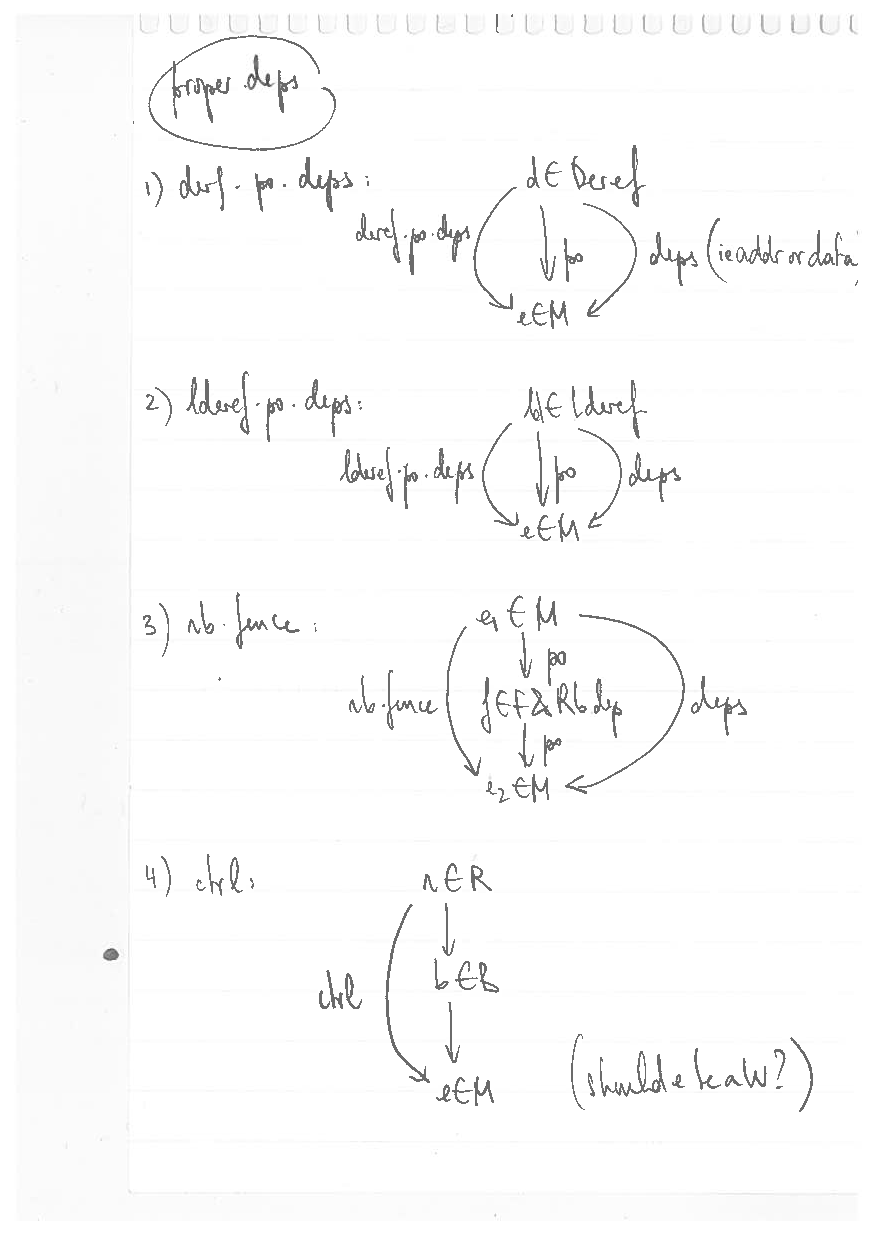
\includegraphics[width=11cm]{proper-deps}

\pagebreak

In the {\tt local} relation we gather our proper dependencies, and all
relations induced by fences, e.g. between two reads in program order separated
by a read memory barrier {\tt 'rmb}, or between two events in program order
separated by a full memory barrier {\tt 'mb}:
\begin{verbatim}
let local = proper-deps | fences
\end{verbatim}

Now we can use all these bricks to build our non-transitive stitch; a
non-transitive stitch is made of one step of the {\tt local} relation (i.e.
proper dependencies or fences), optionally prefixed by a read-from
communication inter-thread:
\begin{verbatim}
let non-transitive = rfe?;local
\end{verbatim}

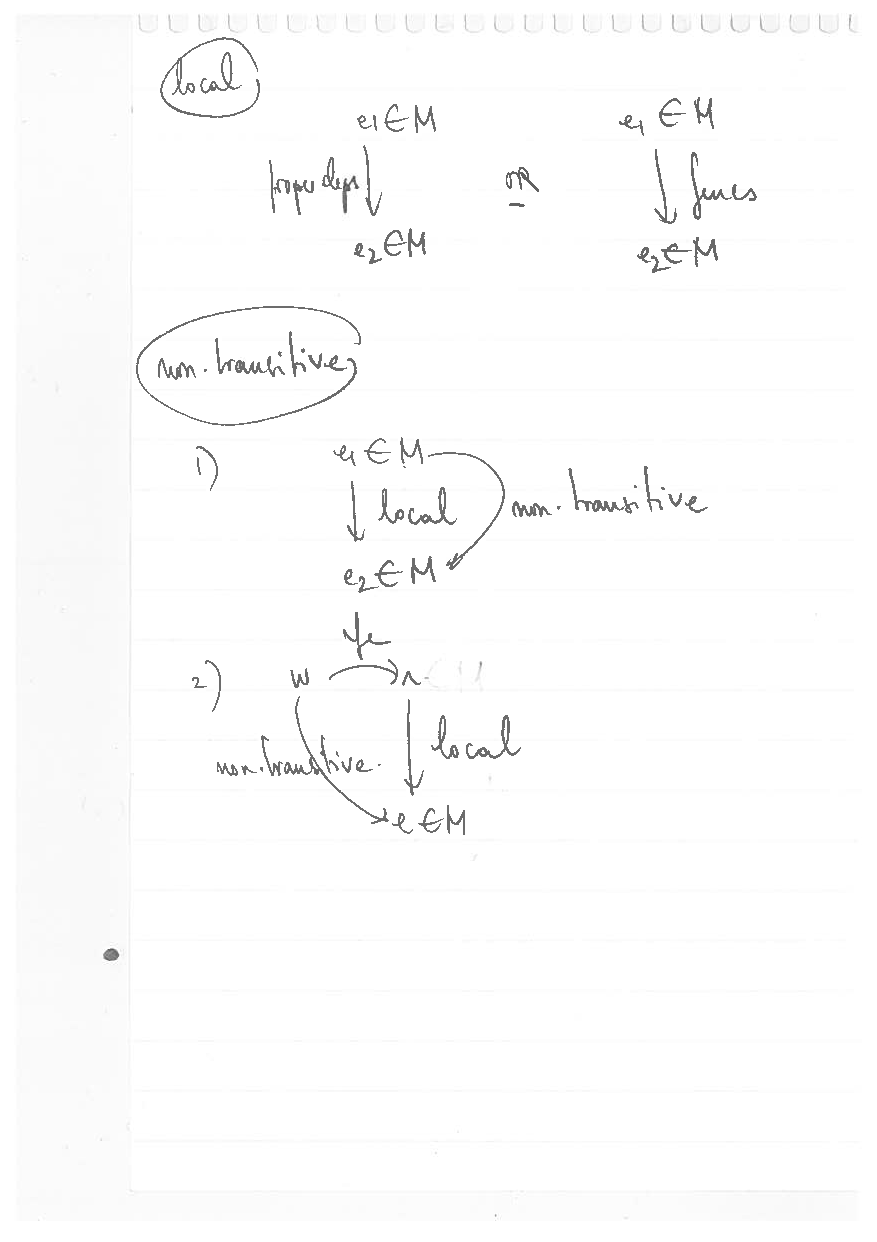
\includegraphics[width=11cm]{local}

\pagebreak

\subsubsection{Pairs, fences and transitive stitches}

The second kind of stitch is \emph{transitive}. It is essentially made of
read-from communication between special accesses, and a fragment of the fences
optionally prefixed by a read-from communication inter-thread. More precisely
we define the relation {\tt pairs} as the union of four kinds of inter-thread
communication over special accesses, and any chain of these four patterns:
\begin{verbatim}
let pairs = ((po?;(rfe & (Release * Acquire));po?) |
            (po?;(rfe & (Assign * Deref));deref-po-deps) |
            (po?;(rfe & (Release * Lderef));lderef-po-deps) |
            (po?;(rfe & (Release * R));ctrl))+
\end{verbatim}

\noindent To understand the {\tt pairs} relation better, it might be helpful to
think of it as instantiating a common pattern four times; viz: \fixme{jade:
perhaps make it a function heh} {\tt r1?;(rfe \& (S1 * S2));r2?}. All four
disjuncts are instances of this pattern, which builds a relation between two
events $e_1$ and $e_2$ such that:
\begin{itemize}
\item $e_1$ is a write which belongs to the set {\tt S1} and $e_2$ a read which
belongs to the set {\tt S2}, such that $e_2$ reads from $e_1$ and they belong
to different threads, or
\item there exists a write $w$ in {\tt S1} which is in {\tt r1} after $e_1$
such that $e_2$ reads from $w$, $e_2$ being a read from the set {\tt S2}, or
\item there exists a read $r$ which belongs to the set {\tt S2} in {\tt r2}
before $e_2$ such that $r$ reads from $e_1$, $e_1$ being a write from the set
{\tt S1}, or
\item there exists a write $w$ from {\tt S1} in {\tt r1} after $e_1$, and there
exists a read $r$ from {\tt S2} in {\tt r2} before $e_2$ such that $r$ reads
from $w$.
\end{itemize}

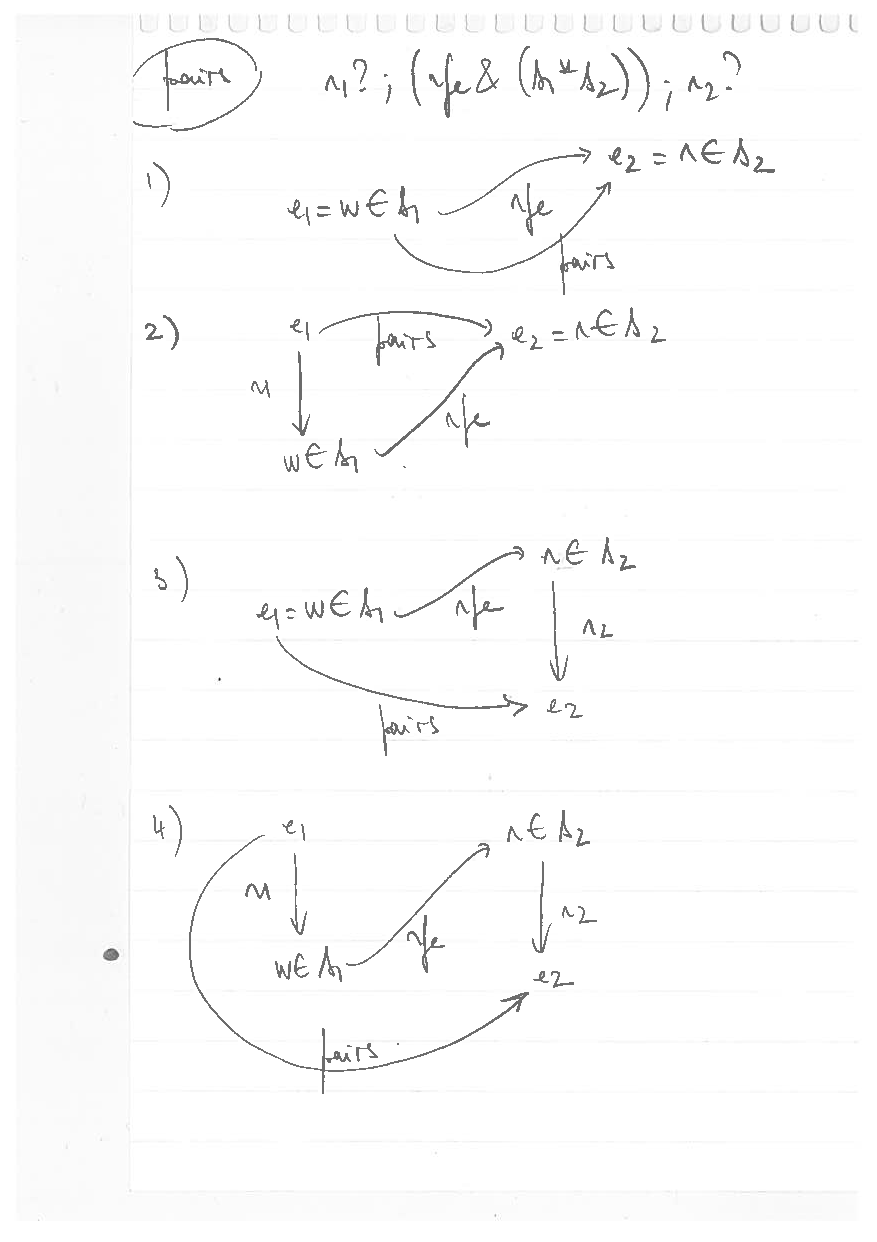
\includegraphics[width=10cm]{pairs1}

\pagebreak

Essentially:
\begin{itemize}
\item the first disjunct pairs write release events to read acquire events
reading from the releases, with one optional step of program order {\tt po}
before the release and after the acquire;
\item the second disjunct pairs write assign events (i.e. {\tt
rcu\_assign\_pointer}) to read deref events (i.e. {\tt rcu\_dereference})
reading from the assigns, with one optional step of program order {\tt po}
before the assign and one mandatory step of {\tt deref-po-deps} after the deref
(i.e. a program order pair starting with a deref event, and also linked by an
address or data dependency);
\item the third disjunct pairs write release events to read lderef events (i.e.
{\tt lockless\_dereference}) reading from the releases, with one optional step
of program order {\tt po} before the release and one mandatory step of {\tt
lderef-po-deps} after the lderef (i.e. a program order pair starting with a
lderef event, and also linked by an address or data dependency);
\item the fourth disjunct pairs write release events to read events reading
from the releases, with one optional step of program order {\tt po} before the
release and one mandatory step of {\tt ctrl} after the read. 
\end{itemize}
\fixme{jade: i.e. a branch? what about read-branch-read, does that count as
ctrl?}

Observe that we wrapped our disjunction of the four pair patterns in a
transitive closure, so that we can chain several of these pairs together (e.g.
first a release-acquire read-from communication, then one step of program
order, then a read-from between an {\tt rcu\_assign\_pointer} and an {\tt
rcu\_dereference} followed by an address dependency).

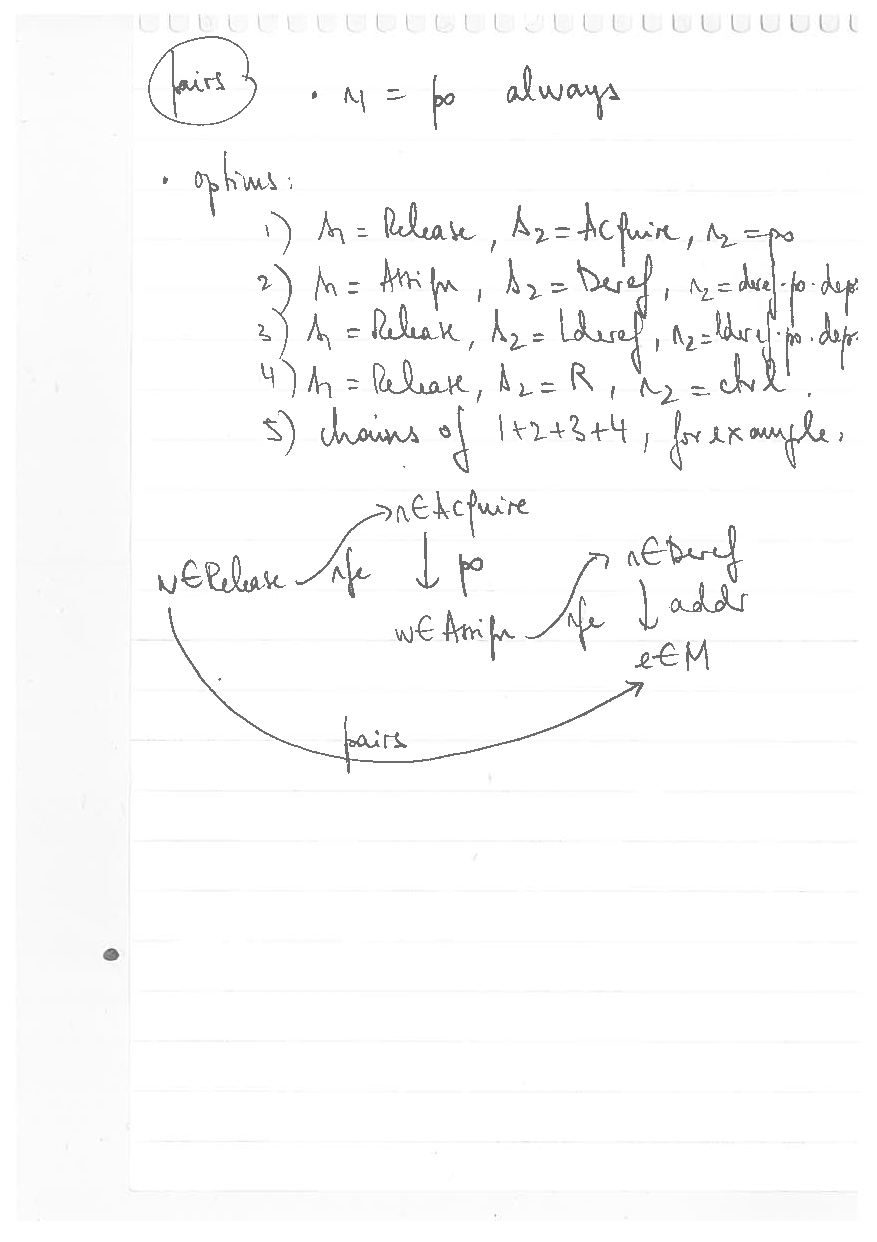
\includegraphics[width=12cm]{pairs2}

%To make the exposition more concrete, let's take a closer look at the first
%disjunct:
%\begin{verbatim}
%po?;(rfe & (Release * Acquire));po? 
%\end{verbatim}
%
%Here we're building a relation between two events $e_1$ and $e_2$ such that:
%\begin{itemize}
%\item $e_1$ is a write release and $e_2$ a read acquire, such that $e_2$ reads
%from $e_1$ and they belong to different threads, or
%\item there exists a write release $w$ in program order after $e_1$ such that
%$e_2$ reads from $w$, $e_2$ being a read acquire, or
%\item there exists a read acquire $r$ in program order before $e_2$ such that
%$r$ reads from $e_1$, $e_1$ being a write release, or
%\item there exists a write release $w$ in program order after $e_1$, and there
%exists a read acquire $r$ in program order before $e_2$ such that $r$ reads
%from $w$.
%\end{itemize}

We also gather the fragment of the fences that ensures transitivity:
\begin{verbatim}
let transitive-fences = (mb | sync)
\end{verbatim}
\noindent where {\tt mb} is the relation by full memory barriers, and {\tt
sync} the relation induced by {\tt synchronize\_rcu}. \fixme{jade: should we
take the transitive closure here in transitive-fences?}

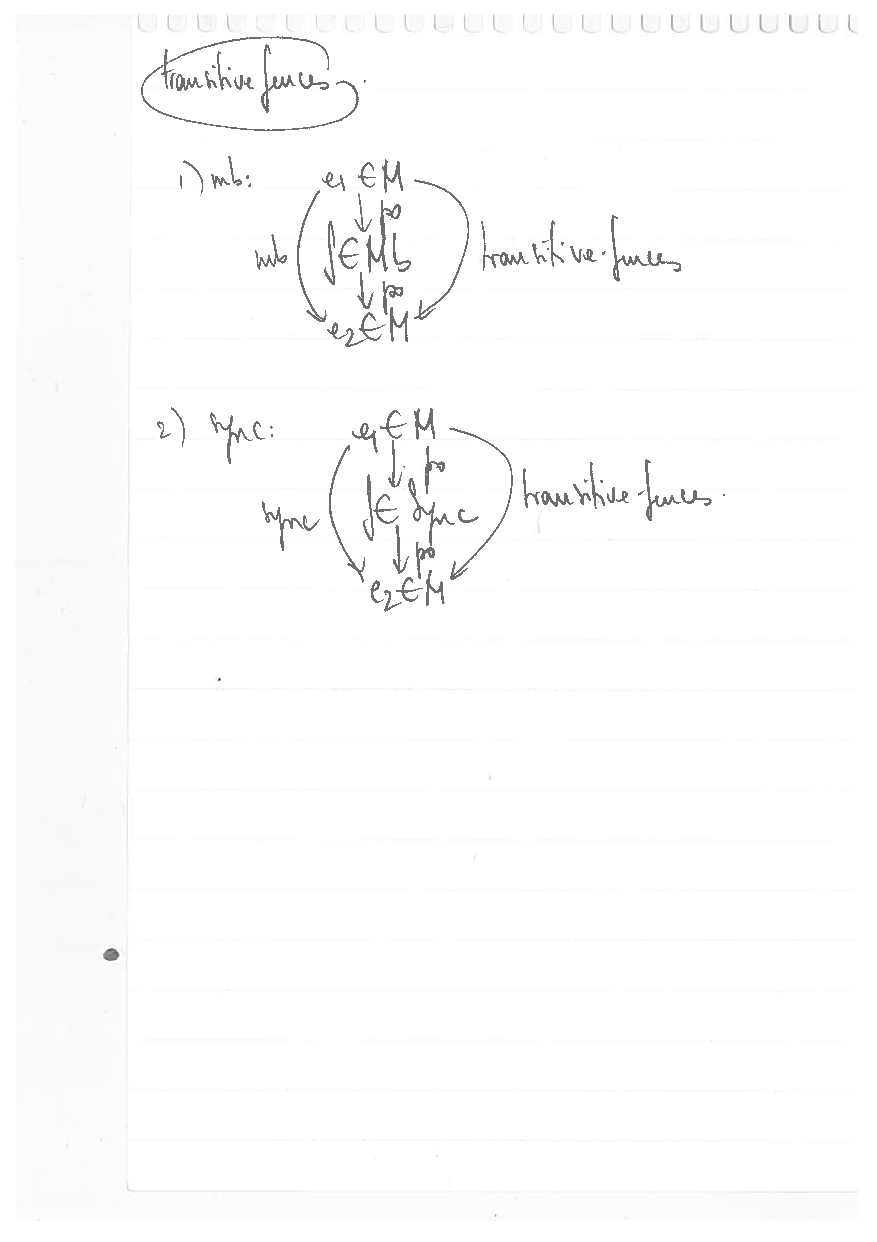
\includegraphics[width=12cm]{transitive-fences}

\pagebreak

Now we can define our transitive stitch as follows:
\begin{verbatim}
let transitive = (rfe?;transitive-fences | pairs)+
\end{verbatim}
\noindent that is, chains of the following components:
\begin{itemize}
\item one step of transitive fence ({\tt mb} or {\tt sync}), optionally
prefixed by an inter-thread read-from communication\fixme{jade: i think so at
least}, or 
\item a chain of special read-from pairs. 
\end{itemize}

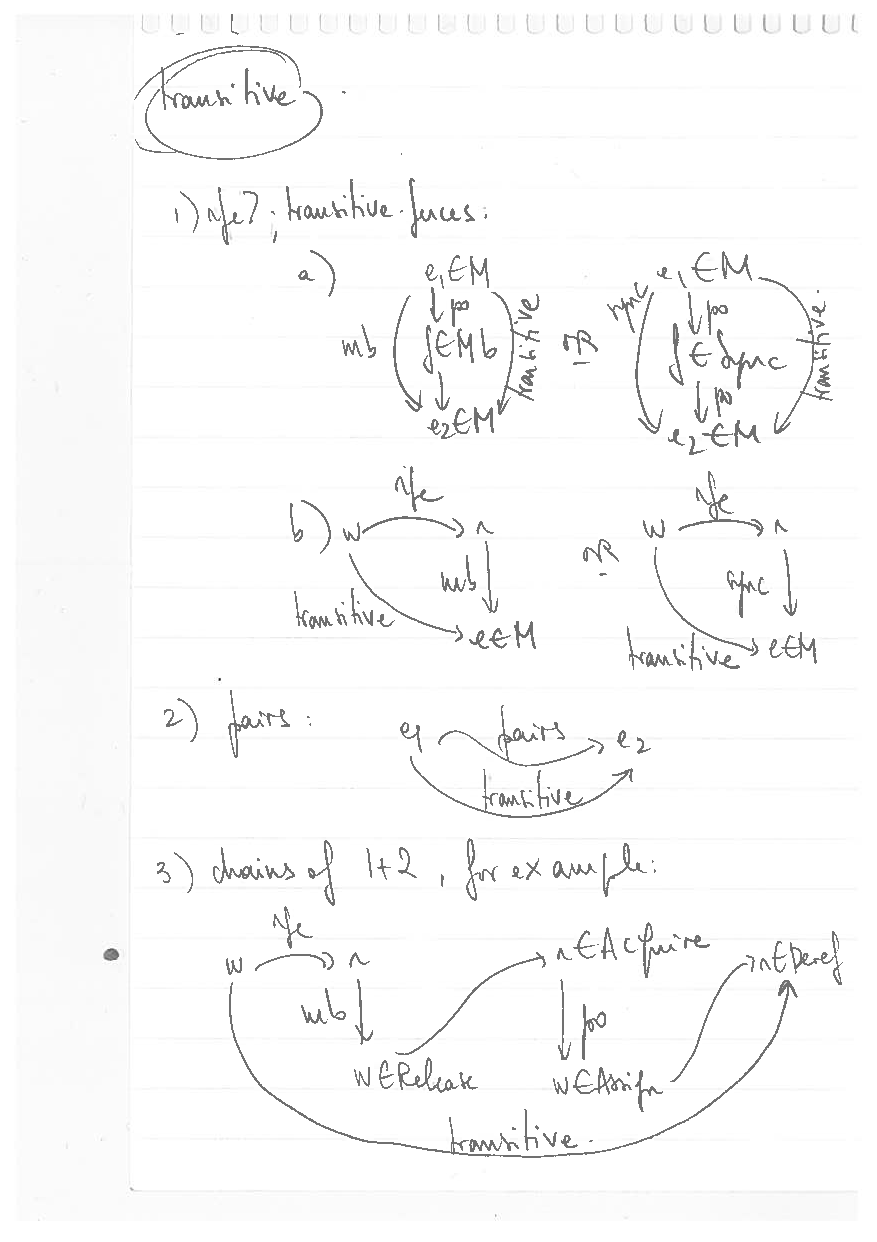
\includegraphics[width=12cm]{transitive}

\pagebreak

\subsection{Happens Before, Causality and Observation}

Our two kinds of stitches let us define the happens-before relation, as
follows:
\begin{verbatim}
let hb = (non-transitive | transitive);non-transitive?
\end{verbatim}

Essentially, the happens-before relation is made of:
\begin{itemize}
\item one step of non-transitive stitch, viz:
  \begin{itemize}
  \item a local ordering such as a proper dependency or a fence;
  \item optionally prefixed by an inter-thread read-from.
  \end{itemize}
\item or one step of transitive stitch, viz chains of:
  \begin{itemize}
  \item chains of special read-from pairs, or
  \item one step of transitive fence (i.e. full memory barrier {\tt mb} or {\tt
synchronize\_rcu}), optionally prefixed by an inter-thread read-from.
\fixme{jade: define A-cumulativity and use this concept everywhere to factor
out this 'optionally prefixed by an inter-thread read-from'}
  \end{itemize}
\end{itemize}

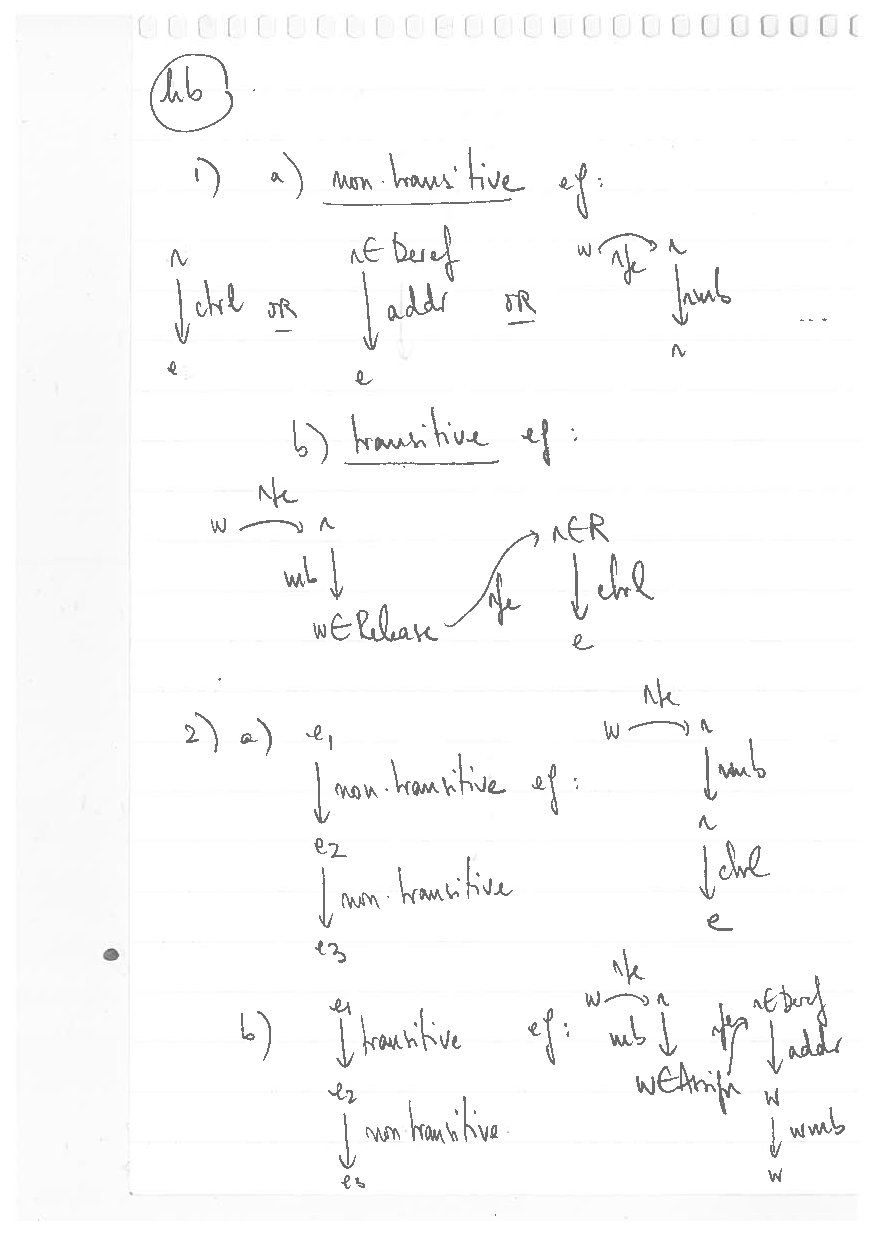
\includegraphics[width=12cm]{hb}

\pagebreak

Now, using the happens-before relation we can state two of the axioms of the
Linux model, viz {\tt causality} and {\tt observation}.

The {\tt causality} procedure requires the happens-before relation to be
irreflexive\fixme{jade: irreflexive?}, which essentially forbids {\tt LB}
shaped examples:
\begin{verbatim}
procedure causality() =
  irreflexive hb
end
\end{verbatim}

The {\tt observation} procedure requires the happens-before relation to not go
against {\tt fre}, which essentially forbids {\tt MP} shaped examples:
\begin{verbatim}
procedure observation() =
  irreflexive fre;hb
end
\end{verbatim}

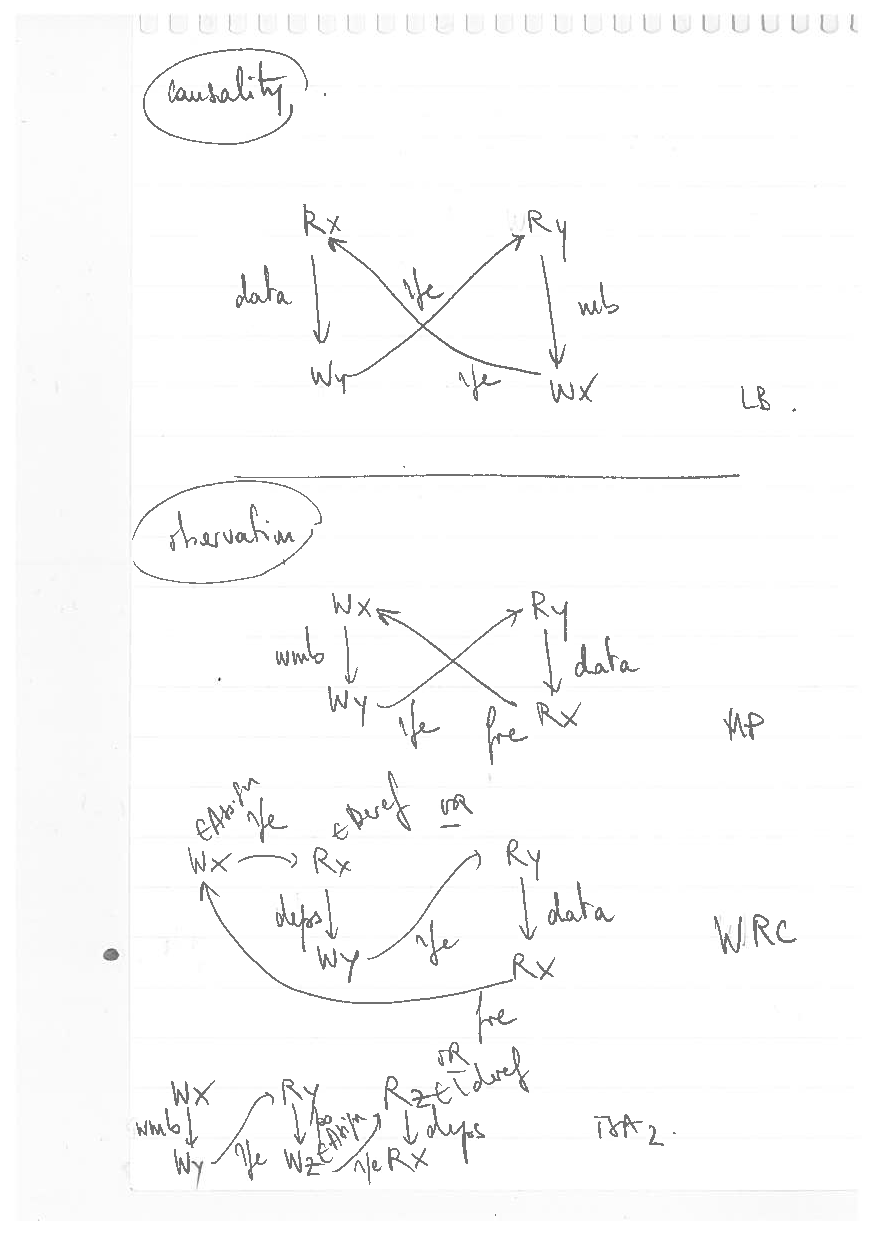
\includegraphics[width=12cm]{c+o}

\pagebreak

\subsection{Propagation}

Our two stitches also let us define the propagation order {\tt prop}:
\begin{verbatim}
let prop = transitive;non-transitive?
\end{verbatim}

\noindent Essentially, the propagation order is made of:
\begin{itemize}
\item one step of transitive stitch, viz chains of:
  \begin{itemize}
  \item chains of special read-from pairs, or
  \item one step of transitive fence (i.e. full memory barrier {\tt mb} or {\tt
synchronize\_rcu}), optionally prefixed by an inter-thread read-from.
\fixme{jade: define A-cumulativity and use this concept everywhere to factor
out this 'optionally prefixed by an inter-thread read-from'}
  \end{itemize}
\item optionally followed by one step of non-transitive stitch, viz:
  \begin{itemize}
  \item a local ordering such as a proper dependency or a fence;
  \item optionally prefixed by an inter-thread read-from.
  \end{itemize}
\end{itemize}

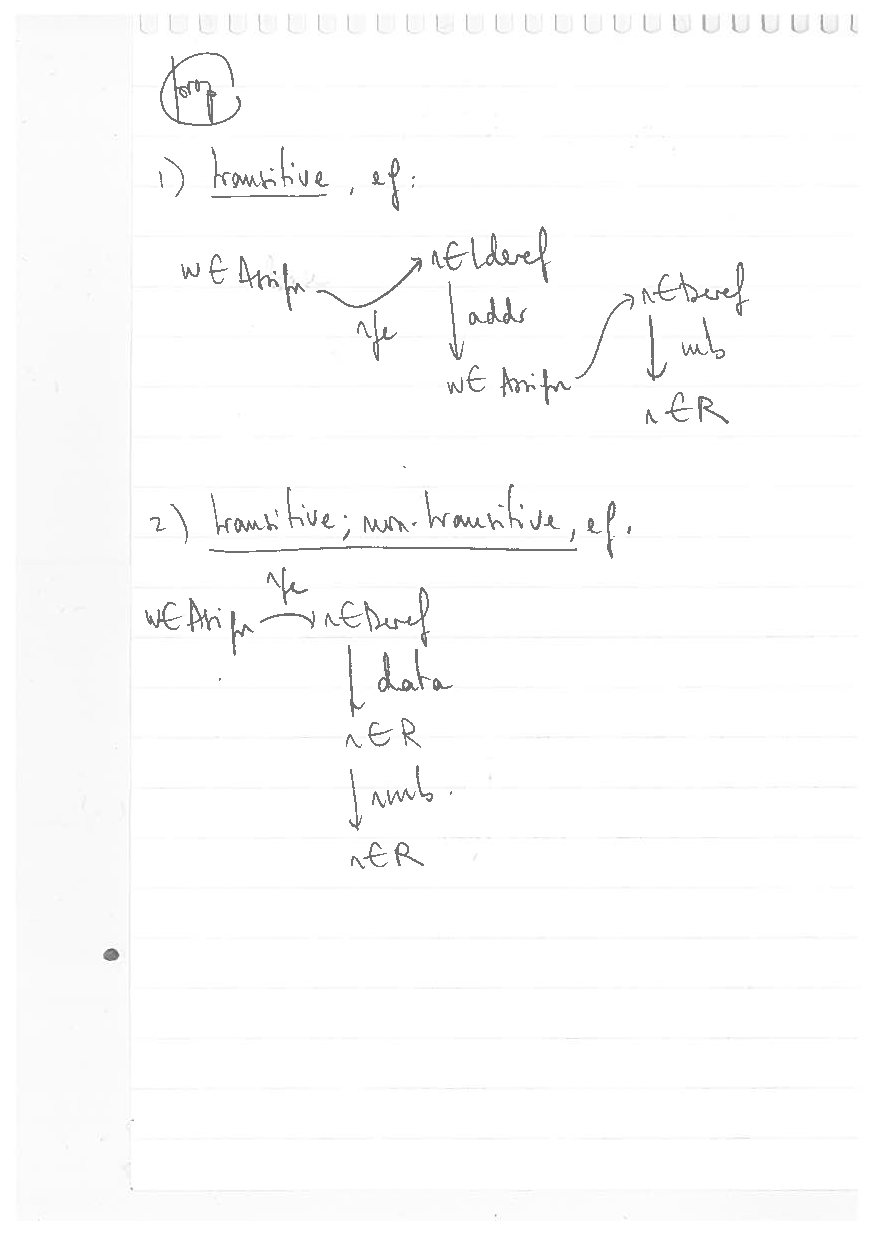
\includegraphics[width=12cm]{prop}

\pagebreak

Now, we can state another axiom of our Linux model. The following {\tt
propagation} procedure requires the coherence order {\tt co} and the
propagation order {\tt prop} to be in accord:
\begin{verbatim}
procedure propagation() =
  acyclic co | prop
end
\end{verbatim}
\noindent that is, forbid {\tt 2+2w} shaped examples.

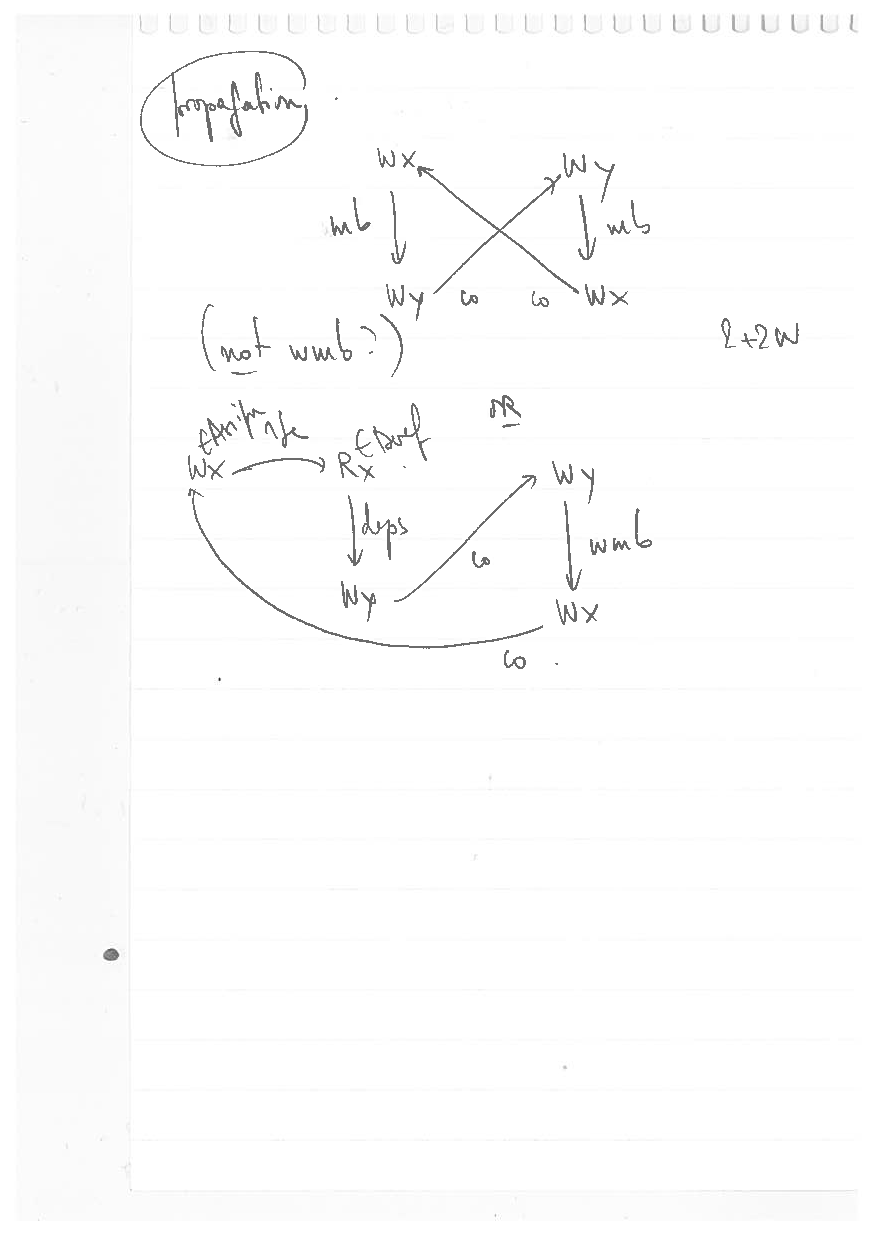
\includegraphics[width=12cm]{propagation}

\subsection{Full memory barriers, RCU grace, and restoring SC}

\subsubsection{Restoring SC with full memory barriers}

In our Linux model, using full memory barriers everywhere restores SC:
\begin{verbatim}
acyclic mb | com
\end{verbatim}
\fixme{jade: say that sc=acyclic po u com} 

\pagebreak

\subsubsection{RCU grace}

We define the RCU grace period as the combination of an {\tt
rcu\_read\_unlock}-{\tt rcu\_read\_unlock}\fixme{jade: read unlock?} sandwich,
and a {\tt synchronize\_rcu}. 

More precisely, we define the relation {\tt between} to gather events that are,
in program order, both after an {\tt rcu\_read\_lock} and before an {\tt
rcu\_read\_unlock}:\fixme{jade: read unlock?}\fixme{jade: also mention nested
sandwiches}
\begin{verbatim}
let between = range(lock-po) & domain(po-unlock)
\end{verbatim}

Now, a {\tt sandwich} is a pair of events either in program order or one step
backwards of program order (i.e. {\tt po\^-1}) that are in the {\tt between}
relation, i.e. between a {\tt lock} and an {\tt unlock}: \fixme{jade:
presumably should be the same lock/unlock pair no? if yes this isn't the case
for now}
\begin{verbatim}
let sandwich = (po | po^-1) & between*between
\end{verbatim}

Now we can define an RCU grace period as follows; the {\tt grace} relation
takes chains of {\tt synchronize\_rcu} followed by any communication {\tt com},
then chains of sandwiches followed by any communication {\tt com}:
\begin{verbatim}
let grace = (sync;com+)+;(sandwich;com+)+
\end{verbatim}

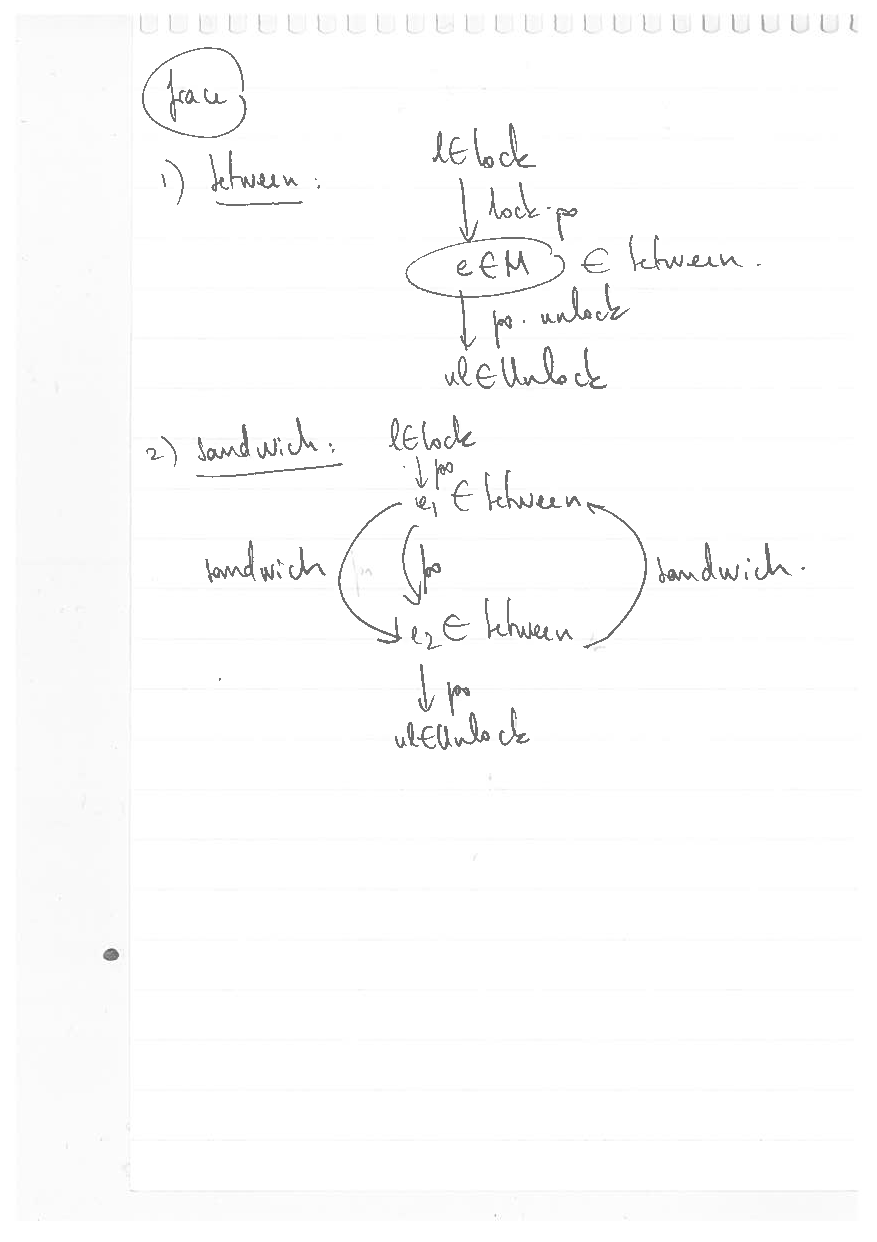
\includegraphics[width=12cm]{grace}

\pagebreak

\subsubsection{Restoring SC: two means}

Finally, our Linux model restores SC by one of two means:
\begin{verbatim}
procedure restoring-sc() =
  acyclic mb | com
  acyclic grace
end
\end{verbatim}
\noindent indeed the procedure {\tt restoring-sc} requires the acyclicity of
the full barrier {\tt mb} with the communications {\tt com}; alternatively,
using RCU's grace period is another way of restoring SC (it enforces more
though).

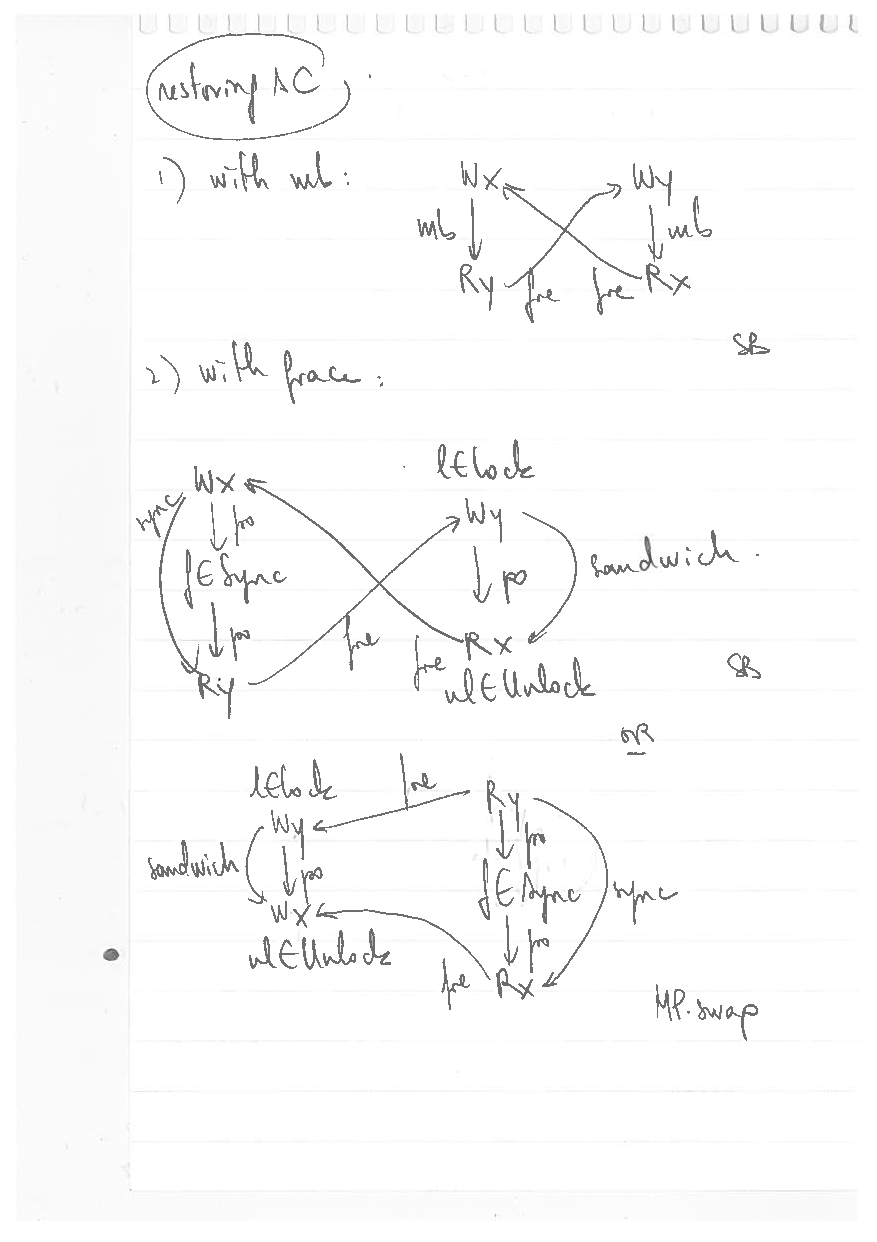
\includegraphics[width=12cm]{sc}

\pagebreak

\section{Seamstresses en folie (cheat sheet)}

Our Linux model is made of two kinds of \emph{stitches} (i.e. combinations of
relations): non-transitive and transitive ones. We use our stitches in various
ways to build the two main relations of our model, namely the happens-before
relation {\tt hb}, and the propagation order {\tt prop}. We recall and
illustrate all these constructs here.

\subsection{Non transitive stitches}

Non transitive stitches are made of local steps (i.e. a proper dependency or a
fence; see Sec.\ref{sec:local}), optionally prefixed by an inter-thread
read-from communication:

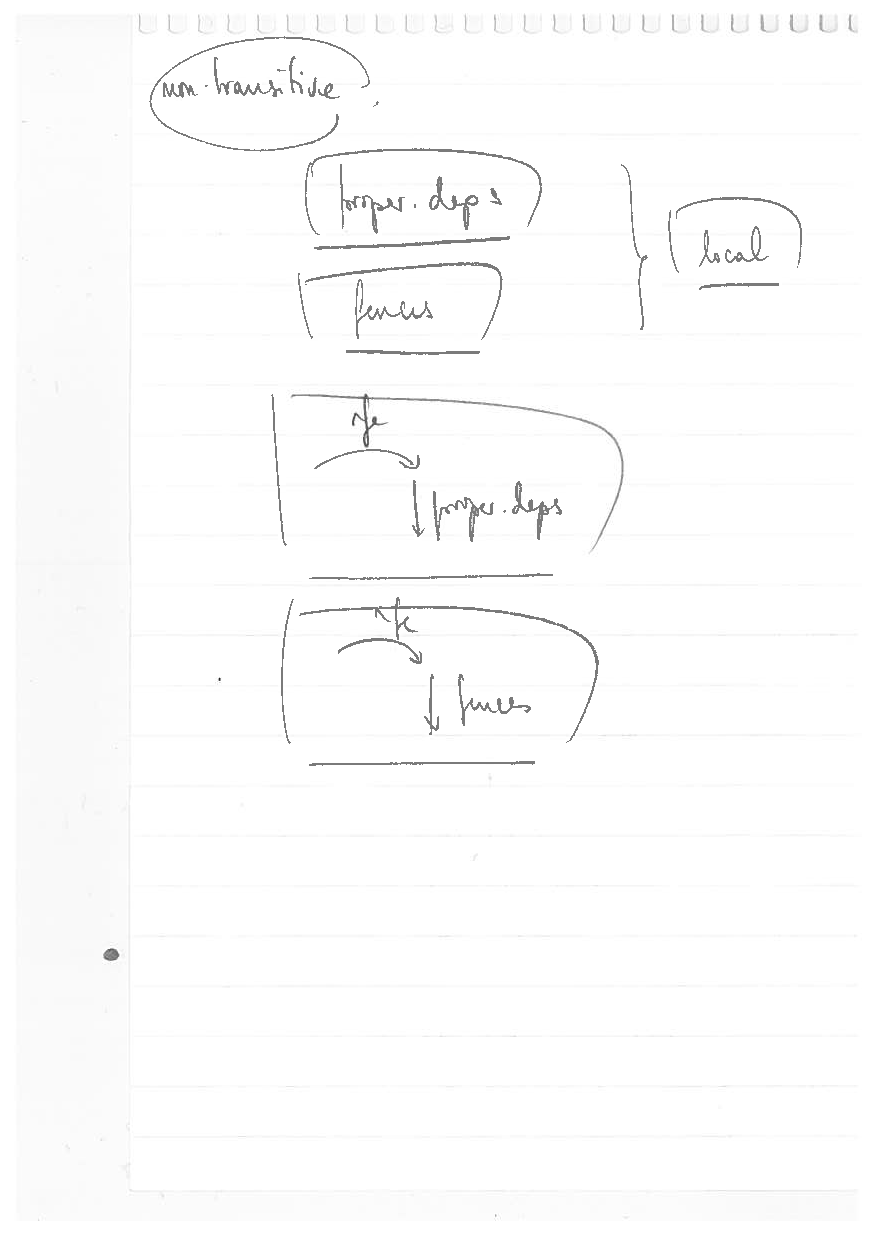
\includegraphics[width=12cm]{non-trans-stitch}

\pagebreak

\subsection{Transitive stitches}

The second kind of stitch is \emph{transitive}. It is essentially made of
read-from communication between special accesses, and a fragment of the fences
optionally prefixed by a read-from communication inter-thread.

\subsubsection{Pairs}

More precisely we define the relation {\tt pairs} as the union of four kinds of
inter-thread communication over special accesses, and any chain of these four
patterns:

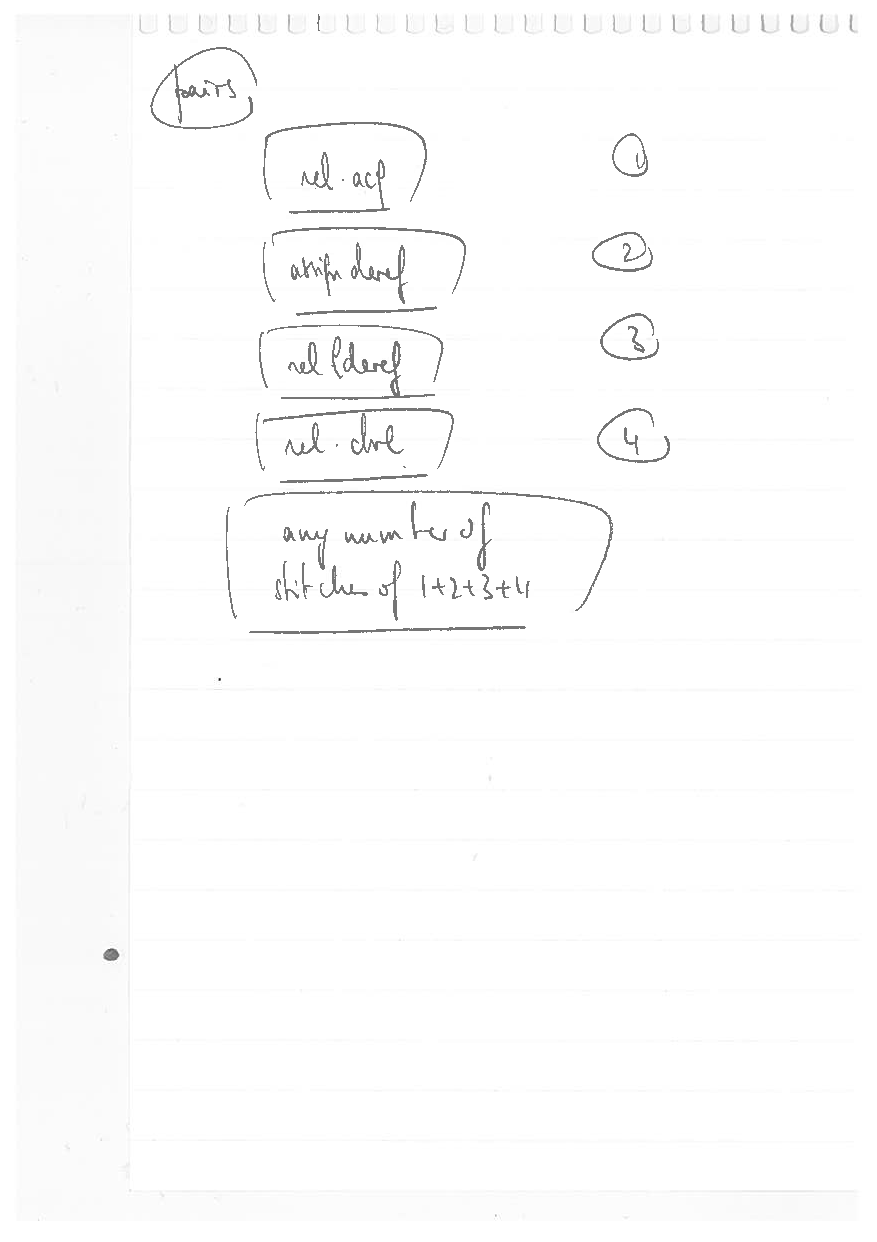
\includegraphics[width=12cm]{pairs-stitch}

\pagebreak

\subsubsection{Transitive stitches}

A transitive stitch is made of a step of transitive fence, optionally prefixed
by an inter-thread read-from communication, or any chain of pairs, or any chain
of these three patterns:

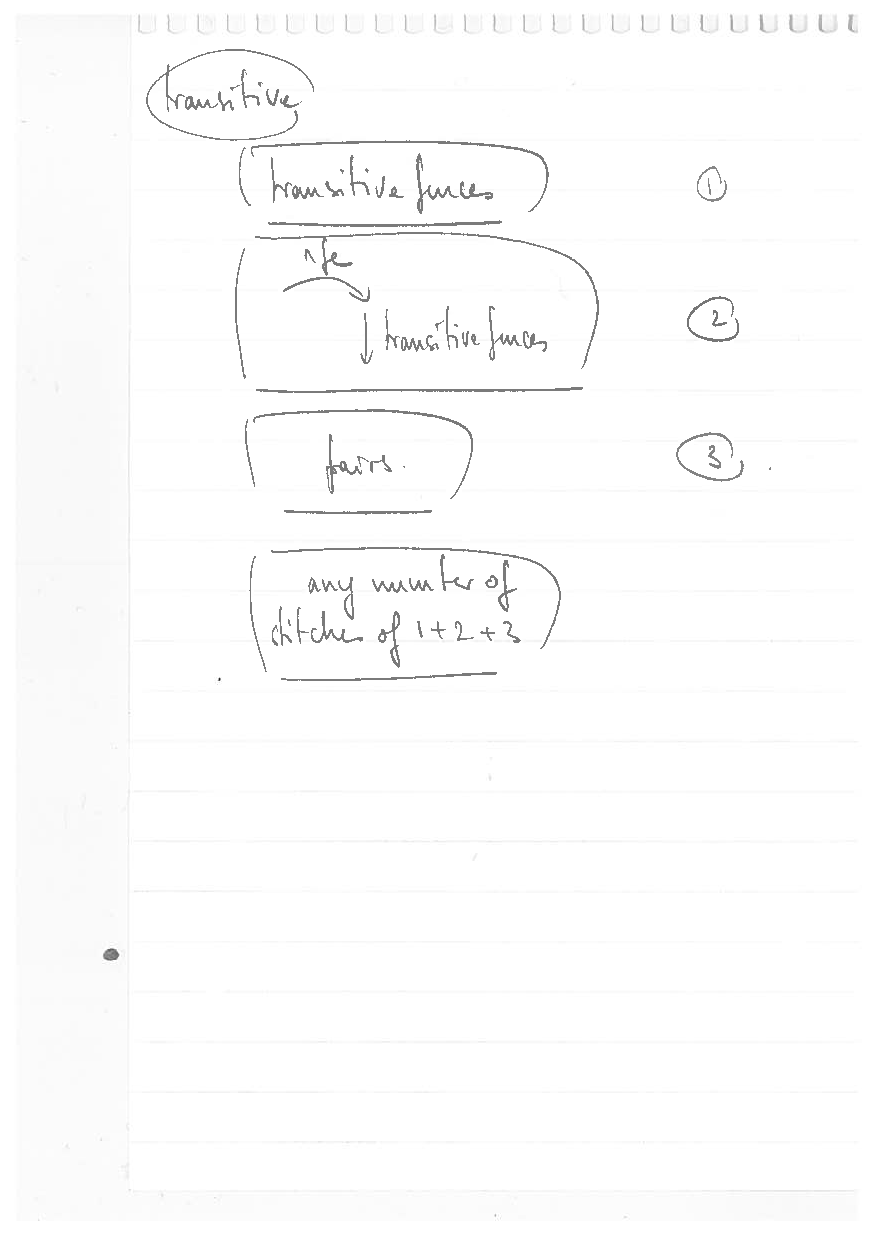
\includegraphics[width=12cm]{trans-stitch}

\pagebreak

\subsection{Happens before}

The happens-before relation is made of one step of non-transitive stitch, or
one step of transitive stitch, or two steps (but no more) or non-transitive
stitches, or one step of transitive stitch followed by one (but no more)
non-transitive stitch:

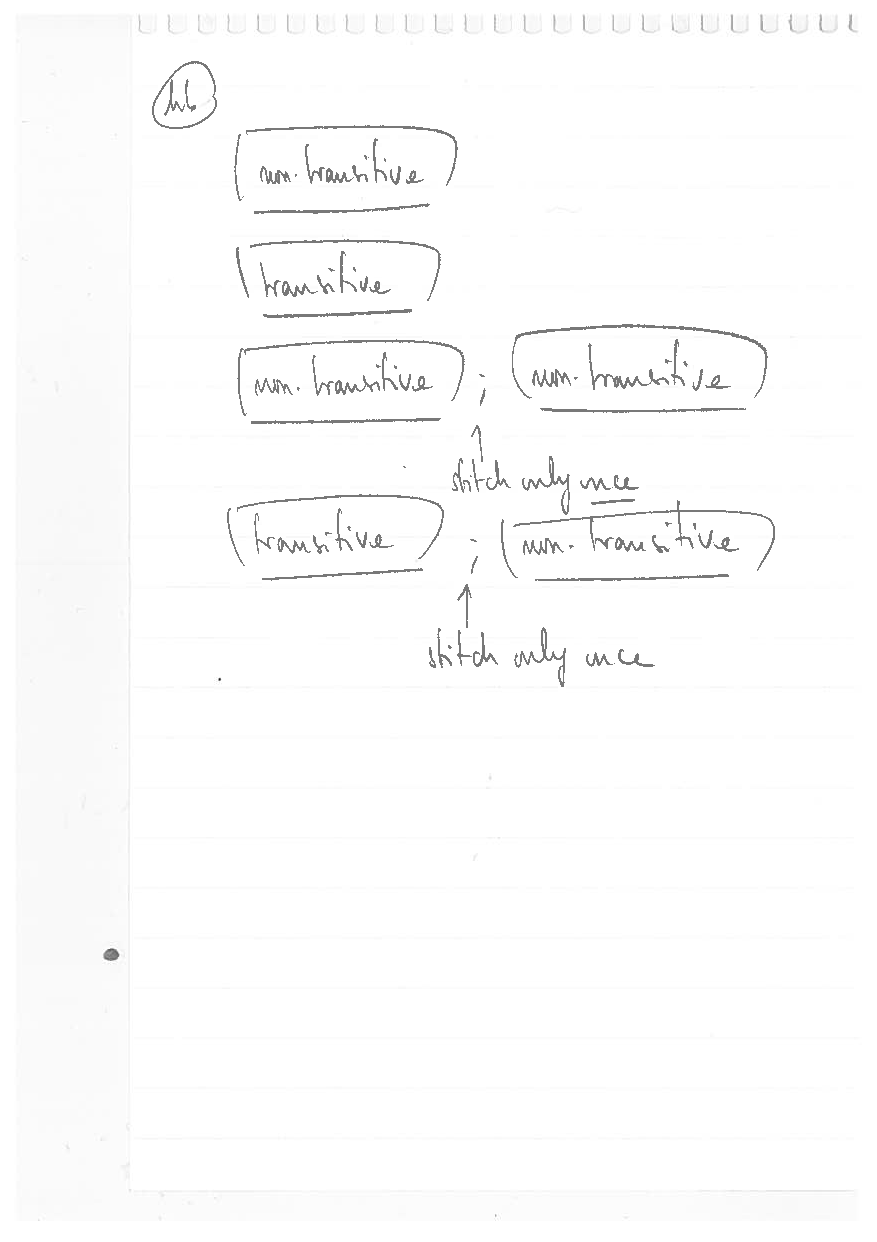
\includegraphics[width=12cm]{hb-stitch}

\pagebreak

\subsection{Propagation}

The propagation relation is made of one step of transitive stitch (which of
course can contain chains), optionally followed by one (but no more) step of
non-transitive stitch:

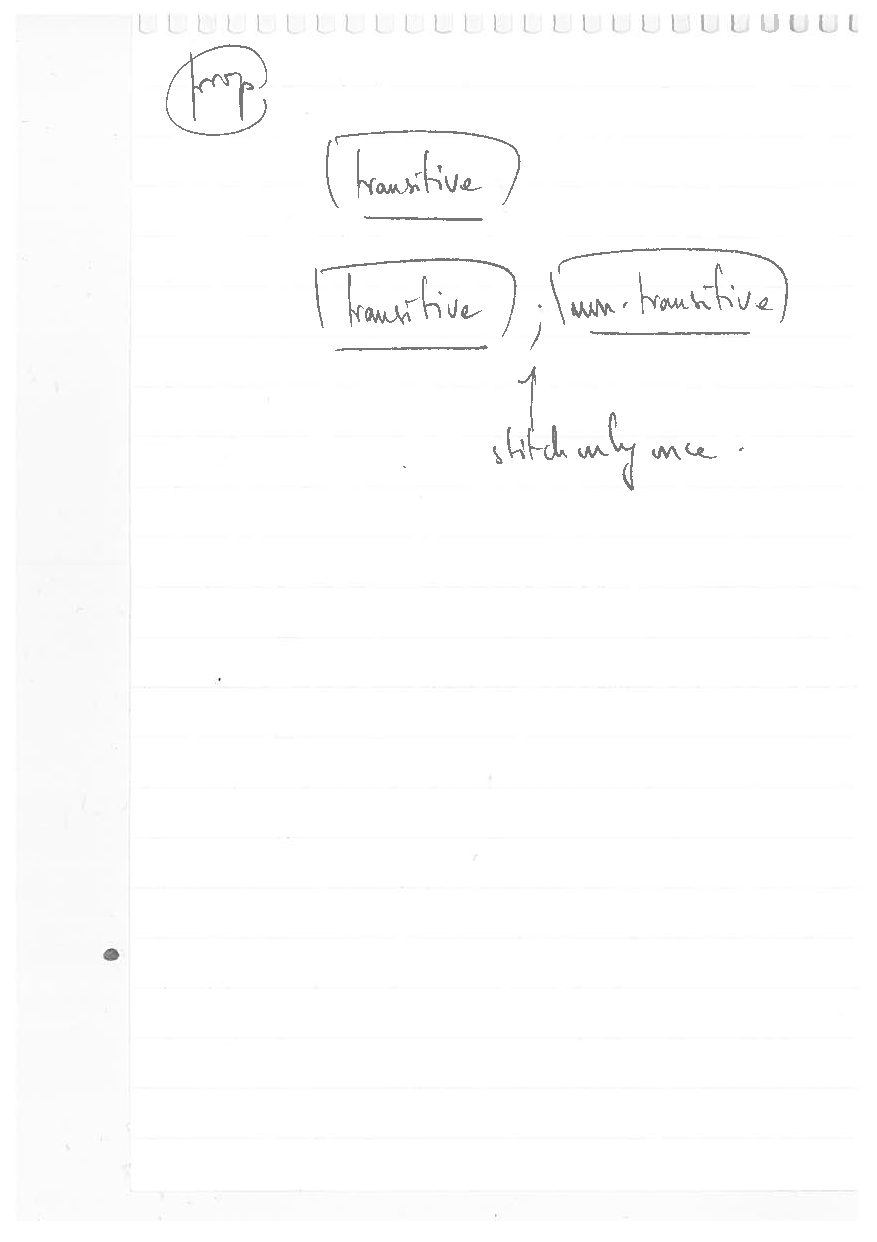
\includegraphics[width=12cm]{prop-stitch}

\end{document}
